\begin{frame}\frametitle{Геометрия и 3D-объекты}
    \begin{itemize}
        \item Придумать внутреннее представление 3D-моделей
        \pause
        \item Научиться читать файлы в формате OBJ
        \item \url{http://www.martinreddy.net/gfx/3d/OBJ.spec}
        \pause
        \item Разобраться с моделью камеры с точечной диафрагмой
        \item Multiple View Geometry in computer vision (Richard Hartley, Andrew Zisserman)
        \pause
        \item Научиться по информации об объекте и камере находить прообраз точки на картинке
        \pause
        \item Научиться по информации об объекте и камере находить контур проекции, видимые рёбра
    \end{itemize}
\end{frame}

\begin{frame}\frametitle{Формат OBJ}
    \begin{itemize}
        \item Это довольно простой, но популярный формат описания геометрических объектов
        \pause
        \item \texttt{v 0.123 0.234 0.345 1.0 \# так описывается точка}
        \item \texttt{f 6/4/1 3/5/3 7/6/5 \# так может описываться грань}
        \item \texttt{f 6 3 7 \# а это то, что нам в действительности от неё нужно}
    \end{itemize}
\end{frame}

\begin{frame}\frametitle{Внутренее представление}
    \begin{itemize}
        \item Камера задаётся матрицей перехода из мировой системы координат в её систему координат и матрице проекции
        \pause
        \item Объект задаётся набором точек и граней в собственной системе координат и матрицей перехода в мировую систему координат
        \item Все геометрические расчёты с участием объекта (поиск пересечений объекта с лучами, поиск видимых рёбер и т.д.) производятся в системе отсчёта объекта. Это удобно т.к., например, позволяет предподсчитать нормали граней.
    \end{itemize}
\end{frame}

\begin{frame}\frametitle{Честная геометрия и эвристики}
    \begin{itemize}
    \item Для поиска прообраза точки луч, соответствующий всем точкам, которые проектируются в данную точку, пересекают с моделью объекта. Среди всех пересечений находится ближайшее к камере
        \pause
        \item "Видимыми" гранями считаются те, которые повёрнуты к камере лицевой стороной
        \pause
        \item "Видимыми" рёбрами считаются те, соседние грани которых видимы
        \pause
        \item Ребро считается лежащим на границе проекции, если видна ровно одна из соседних граней
        \pause
        \item Находить видимые грани можно одним проходом по списку граней с $O(1)$ вычислений для каждой грани
        \item Эти эвристики абсолютно точно работают на выпуклых объектах и довльно неплохо для близких к выпуклым
    \end{itemize}
\end{frame}

\begin{frame}\frametitle{Работа эвристик}
    \begin{center}
        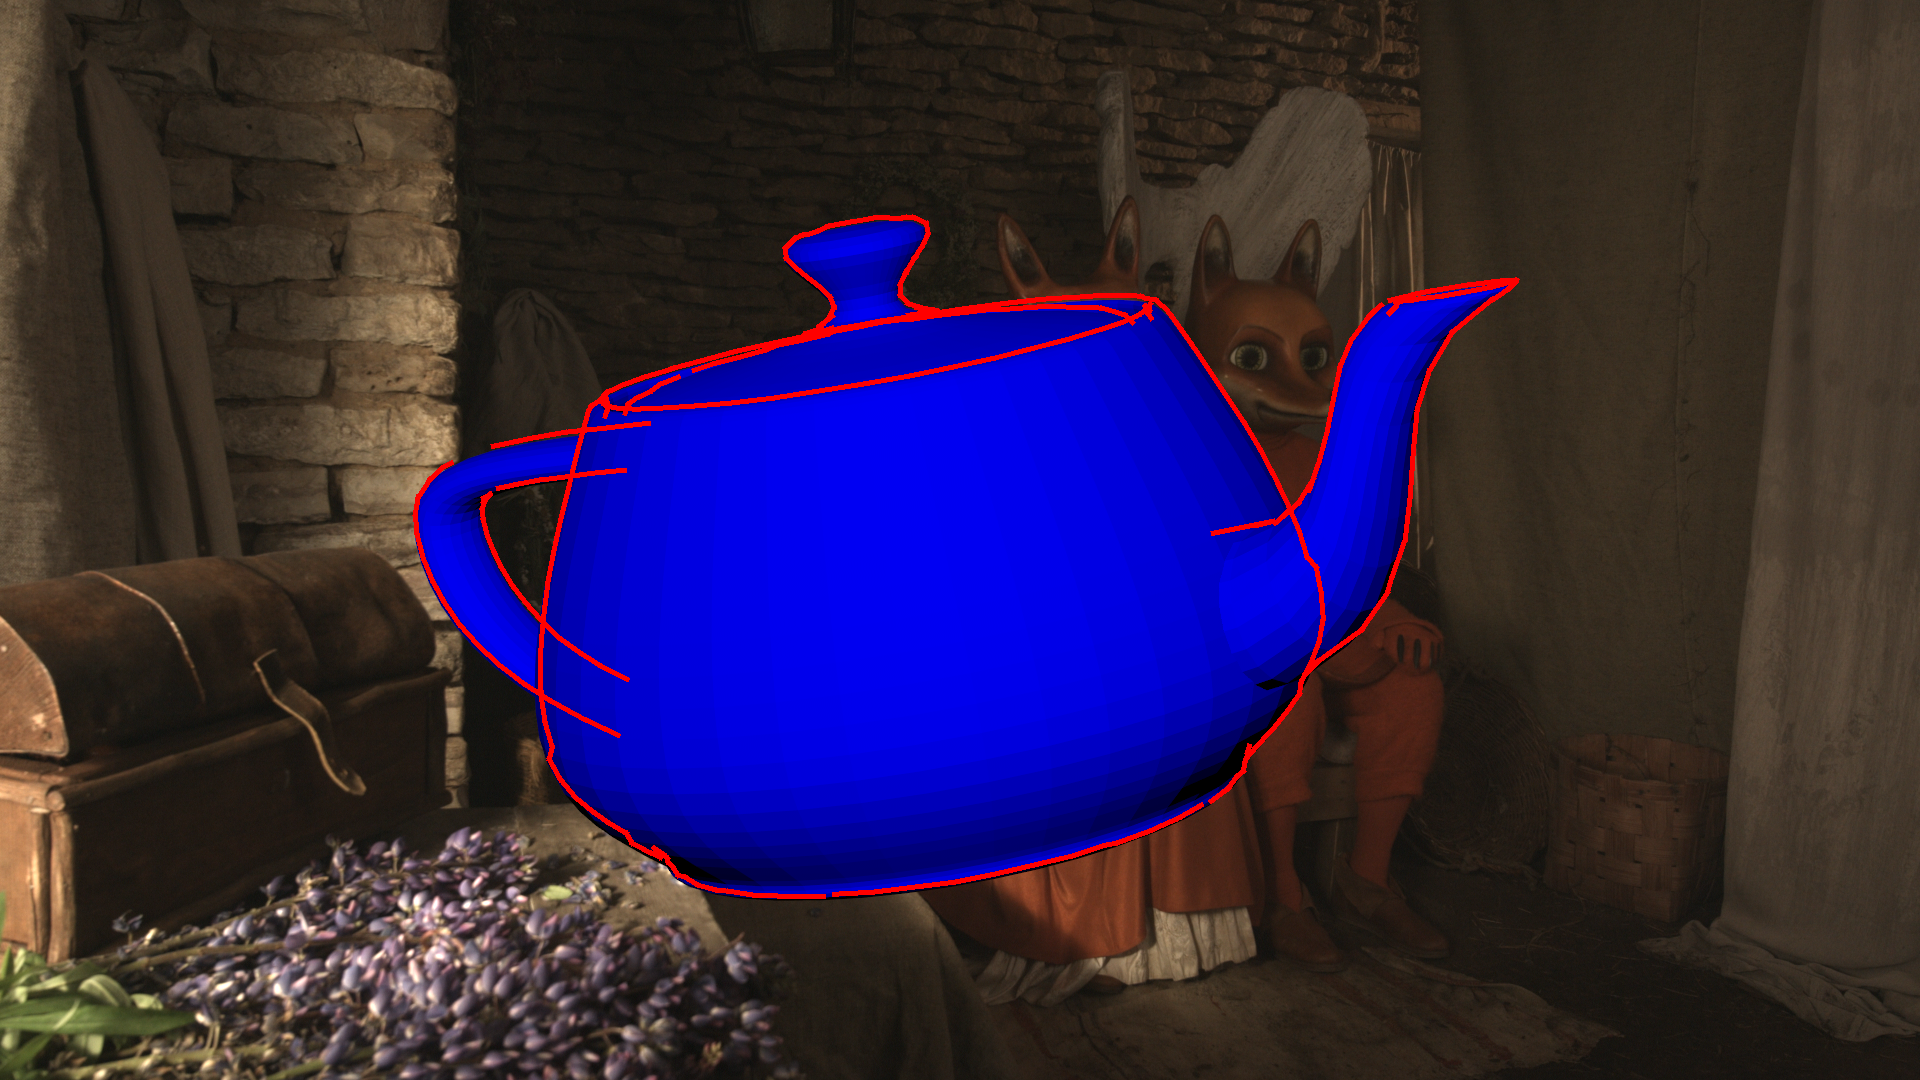
\includegraphics[height=6cm]{lobanov_imgs/border.png}
    \end{center}
\end{frame}

\begin{frame}\frametitle{Работа эвристик}
    \begin{center}
        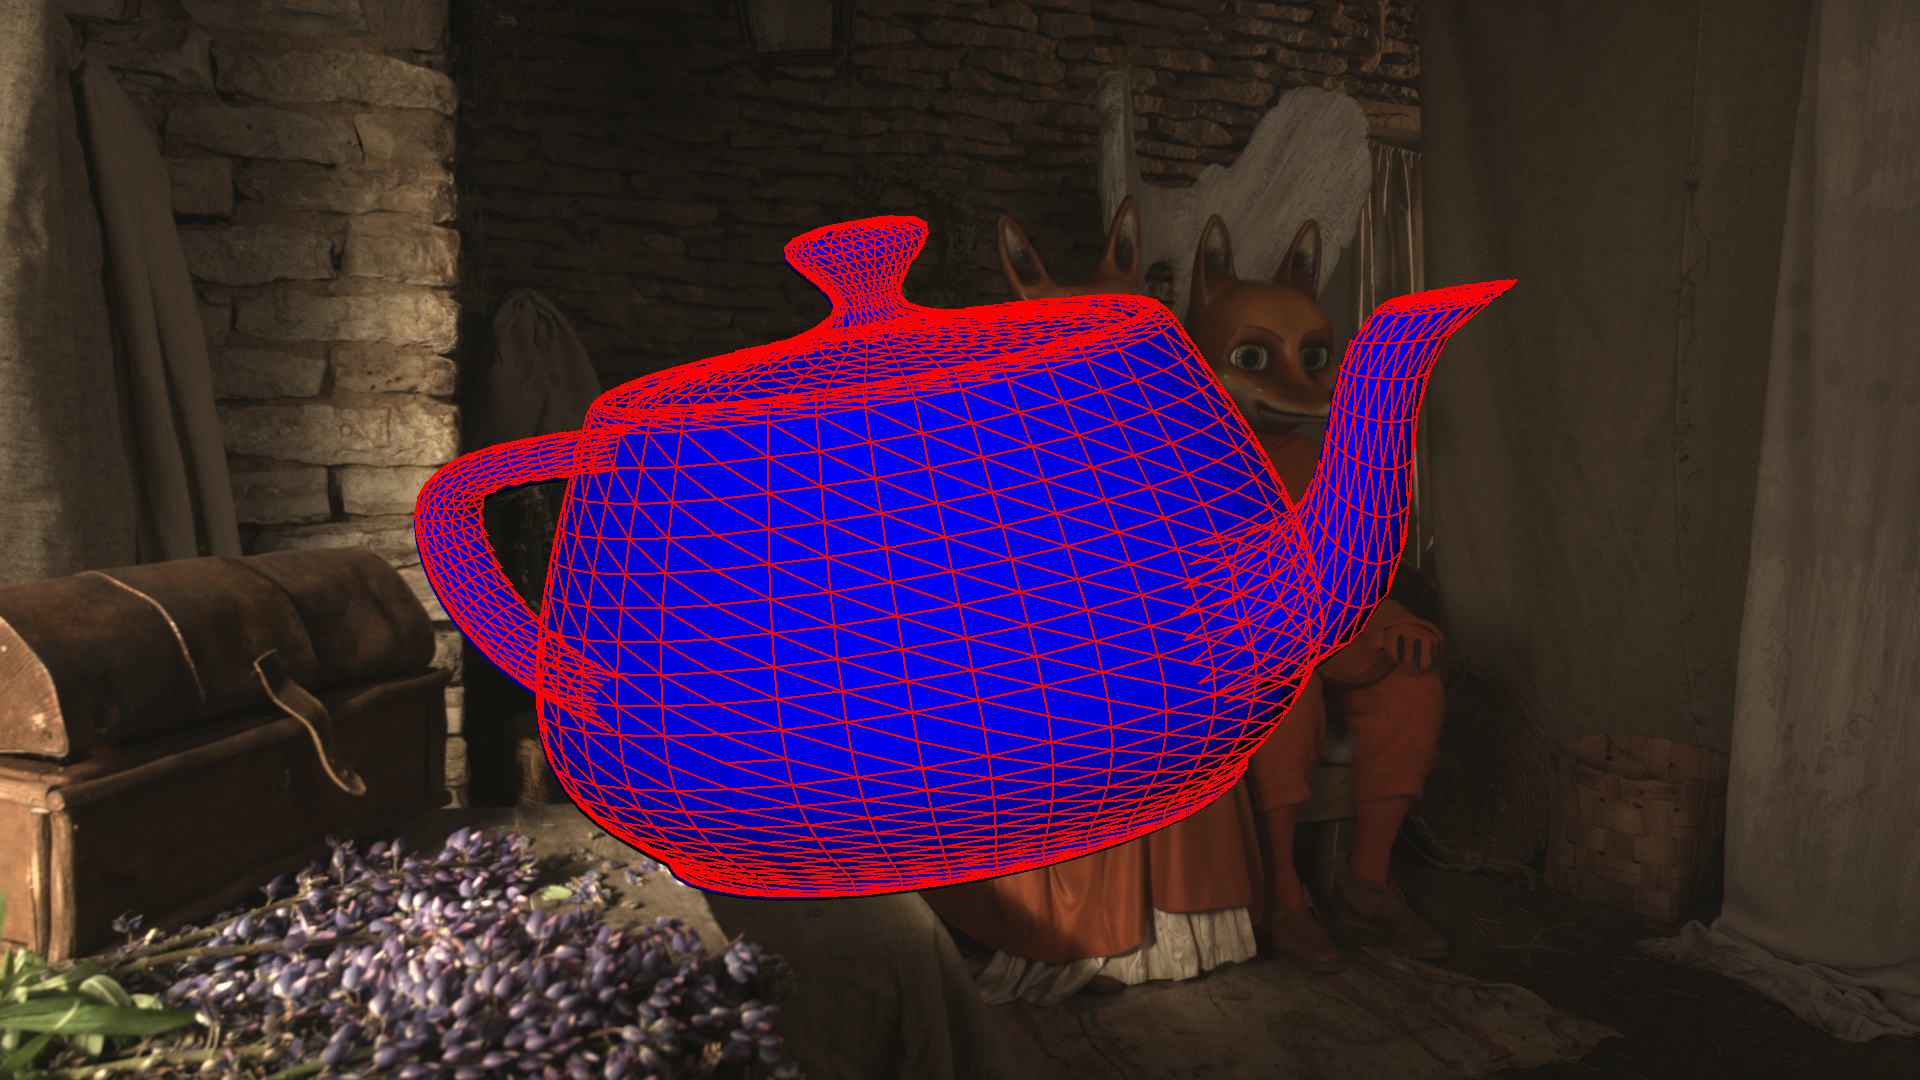
\includegraphics[height=6cm]{lobanov_imgs/visible_edges.png}
    \end{center}
\end{frame}

\begin{frame}\frametitle{numpy}
    \begin{itemize}
    \item Библиотека numpy позволяет создавать массивы примитивных типов в python
        \item В нашем проекте используется для компактного хранения точек и для ускорения операций, применяемых к большому количеству точек
    \end{itemize}
\end{frame}
